\documentclass[a4paper]{scrartcl}

\usepackage[ngerman]{babel}
\usepackage[T1]{fontenc}
\usepackage[utf8]{inputenc}  % Umlaute etc. verwenden
\usepackage[final]{graphicx}    % Grafiken einbinden
\usepackage{url}
\usepackage[nodayofweek,level]{datetime}


\usepackage[pdftex,
    pdftitle={Ein Vergleich zwischen der Umsetzung verschiedener Konzepte in Fuchsia, ChromeOs und Android},
    pdfauthor={Niklas Weimann}]{hyperref}


\setcounter{secnumdepth}{3}


\begin{document}

% Der Titel der Seminararbeit, sowie der Autor
\title{Ein Vergleich zwischen der Umsetzung verschiedener Konzepte in Fuchsia, ChromeOs und Android}
\author{Niklas Weimann}
\date{\formatdate{4}{7}{2020}}

\maketitle
\tableofcontents
\newpage

\section{Einleitung}
„Pink + Purple == Fuchsia (a new Operating System)“\cite{fuchsia.Gettingstarted} So beschreibt Google ein neues Betriebssystem, das sich zurzeit noch in aktiver Entwicklung befindet. Das genaue Ziel dieses neuen Betriebssystems ist bis jetzt nur Google selbst bekannt, aber es gibt in den Medien einige Spekulationen darüber, wieso dieses System neu entwickelt wird und was die Absicht dahinter sein könnte. Dabei taucht immer wieder die Vermutung auf, dass Fuchsia als Ersatz für die bereits existierenden Betriebssysteme Android und ChromeOS entwickelt wird.\cite{DaveAltavilla.30.Juni2019}

Android und ChromeOS stammen aus dem Hause Google und setzen beide auf  einen Linux Kernel.  ChromeOs ist, vereinfacht zusammengefasst, nur eine Version des Chrome Browsers als Betriebssystem, das durch Browsererweiterungen und Apps um zusätzliche Funktionen ergänzt werden kann. Außerdem bietet ChromeOs die Möglichkeit Android Apps auszuführen. ChromeOs ist speziell auf den Laptop Bereich ausgerichtet und setzt dort seinen Fokus auf Produktivität im Office Bereich. Android hingegen ist auf Smartphones und Tablets ausgerichtet und versucht den gesamten Bereich der mobilen Geräte abzudecken.

Google hat für die Entwicklung des neuen Systems einen Kernel basierend auf dem Littlekernel Projekt entwickelt. Dieser Kernel wird bereits für den Android bootloader \cite{Android.LittleKernel} und das Android Trusted Execution Enviroment \cite{Android.TrustyTee} eingesetzt. Unter Fuchsia wird Littlekernel als Basis für den Microkernel des Systems verwendet. Während Linux auf einen monolithischen Kernel setzt, verwendet Fuchsia einen Mikrokernel, der nur die absolut notwendigsten Funktionen implementiert, alle weiteren Funktionen müssen im Userspace ausgeführt werden. Bedingt durch den unterschiedlichen Kernelansatz von Fuchsia und Android, unterscheidet sich die Systemarchitektur der beiden Systeme stark voneinander. Fuchsia verwendet ebenso nur wenige Systemdienste, somit beschränken sich diese auf ein Komponenten Framework, einen Cloudagent namens Ledger und weitere weniger wichtige Dienste.

Diese Arbeit beleuchtet die wesentlichen Konzepte, in denen sich Fuchsia und Android voneinander unterscheiden. Dazu werden zunächst die wichtigsten Unterschiede zwischen den Kernels der beiden Systeme beleuchten. Anschließend wird ein Überblick, sowie eine Bewertung, des Komponenten Frameworks, das eine zentrale Rolle in Fuchsia spielt, gegeben. Zum Schluss wird die Handhabung von Treibern und die Dateiverwaltung der verschiedenen Systeme verglichen.

\section{Zircon}
Ziron, der Kernel von Fuchsia, ist aus dem Littlekernel Projekt, einem Projekt von Travis Geiselbrecht, entstanden. Littlekernel, sowie Zircon setzten auf den Microkernelansatz, somit ist der Kernel sehr flexibel einsetzbar und kann sowohl in IoT-Hardware als auch Desktop Computern eingesetzt werden.

\subsection{Kernel Objekte und System Calls}
Der Zircon Kernel unterstützt mehr als 150 System Calls, die, bis auf jene zur Synchronisation, asynchron und unterbrechbar sind.  \cite{Fuchsia.Zircon.Systemcalls} Somit ist es möglich, dass ein Prozess oder ein Thread während seiner Ausführung auf eine andere CPU migriert werden kann. Zusammen mit speziell für Zircon optimierte Prozessoren, kann dies für einen besseren Lastausgleich und eine damit verbundene bessere Performance sorgen.

Zircon verwendet Handles, um eine Verbindung zwischen Objekten im Kernel und dem Userspace herstellen zu können. Handles werden von System Calls zurückgegeben, falls diese ein Kernel Objekt erstellt haben (z.b. zx\_event\_create() + zx\_process\_create() + zx\_thread\_create()). Im Usermode ist dieses Handle eine 32 Bit lange Zahl, wobei die letzten 2 LSB bei validen Handles immer gesetzt sind. Ein Handle, dass ausschließlich aus Nullen besteht, ist jedoch stets ein ungültiges Handle. Jedes Handle hat immer nur für den Prozess eine Bedeutung, der es durch die Erstellung eines Kernelobjektes angefordert hat. Während ein Handle in einem Prozess A eine Bedeutung hat und auf ein valides Kernel Objekt zeigt, kann es in einem anderen Prozess ungültig sein, oder auf ein anderes Objekt verweisen, damit die Bedeutung des Handles erhalten bleiben kann, muss dieses über einen System Call an den anderen Prozess übergeben werden. Ein Prozess kann mehrere Handles haben, um auf dasselbe Kernel Objekt zuzugreifen, wobei sich dann meist die jeweiligen Zugriffsrechte unterscheiden. Wird das letzte Handle für ein Kernelobjekt geschlossen, so wird der Kernelobjekt ebenfalls entfernt. \cite{Fuchsia.Zircon.Handles}

Die Zugriffsrechte, die ein Handle auf ein Kernel Objekt hat, werden im Kernel gespeichert. Der Kernel hat für jedes Handle ein C++ Objekt, das erstens eine Referenz auf das Kernel Objekt hat, zweitens eine Liste mit allen Rechten, die das Handle besitzt, und drittens eine Referenz auf den Prozess, zu dem es gehört. Diese Zugriffsrechte können einschränken werden, indem mittels zx\_handle\_duplicate() \cite{Fuchsia.HandleDuplicate} oder mittels zx\_handle\_replace() \cite{Fuchsia.HandleReplace} ein neues Handle erstellt wird, das eine Teilmenge der Rechte des ursprünglichen Handles besitzt. \cite{Fuchsia.Zircon.Handles}

Jedes Kernel Objekt kann eine Reihe an Outputs haben, sogenannte Signale. Jedes Signal kann nur eine ein Bit Information repräsentieren, wobei pro Objekt bis zu 32 Signale möglich sind. Signale können mittels System Calls erwartet werden, sie repräsentieren den Zustand, in dem sich das Kernel Objekt gegenwärtig befindet. \cite{Fuchsia.Zircon.Signals}

Linux besitzt keine Kernel Objekte und keine Handles. Systemcalls unter Linux sind primitiver umgesetzt, es wird bei einem Systemcall kein Handle mitgegeben, durch das geprüft wird ob ein Aufrufer die entsprechenden Rechte hat. Wenn ein Systemcall aufgerufen wird, dann werden die entsprechenden Daten, sowie die Nummer des entsprechenden Systemcalls in definierte Register geschrieben. Durch einen Interrupt Aufruf findet dann ein Wechsel in den Kernelmode statt. Der Kernel überprüft dann basierend auf den Rechten, die diesem Prozess zugewiesen wurden, ob dieser Prozess den entsprechenden System Call aufrufen darf, dazu unterhält der Kernel eine Liste mit allen Rechten, über die die aktuell aktiven Prozesse Verfügen. \cite{Android.Kernel.Capabilities}
\subsection{Scheduling}
Zircon stellt für jede CPU einen unabhängigen Scheduler bereit, jedoch können die Scheduler untereinander kommunizieren, um Überlasten zu erkennen, und Prozesse bei Bedarf auf eine andere CPU migrieren. Außerdem können Prozesse selbst angeben, dass sie auf einer anderen CPU ausgeführt werden sollen.

Jeder Scheduler kann zwischen 32 möglichen Prioritäten unterscheiden und besitzt entsprechend für jede Priorität eine Warteschlange, in der die Prozesse auf die Ausführung warten, solange sie nicht den Status „Blocked“ haben. Ein geblockter Prozess wird in eine Warteschlange für die entsprechende Ressource gepackt und nimmt nicht weiter am Scheduling teil, bis er entblockt wird. Wenn die Ressource frei ist und der Prozess seine Arbeit mit der Ressource verrichtet hat, wird er entblockt und direkt an den Anfang der entsprechenden Warteschlange für seine Priorität eingefügt, sodass er sein komplettes Zeitintervall ausnutzen kann. Hat er das Zeitintervall aufgebraucht, wird er wieder ans Ende der Warteschlange eingefügt. \cite{Fuchsia.Zircon.Scheduling}

Welche Priorität ein Prozess bekommt, hängt dabei von drei Faktoren ab. Erstens gibt es eine Basis Priorität, die frei gewählt werden kann, zweitens gibt es einen Prioritätsboost und drittens eine Prioritätsvererbung.

Der Prioriätsboost wird auf die Basis Priorität addiert. Wird der Prozess entblockt, nachdem er auf eine Ressource gewartet hat, wird seine Prioritätsstufe erhöht, wohingegen die Prioritätsstufe um eins verringert wird, wenn der Prozess vor Ende seines zugewiesenen Zeitintervalls ein Resheduling anfordert oder wenn er das komplette Zeitintervall ohne Unterbrechung gerechnet hat. \cite{Fuchsia.Zircon.Scheduling}

Die Prioritätsvererbung wird eingesetzt, um Prozesse, die auf eine Ressource warten, die jedoch durch den aktuellen Prozess blockiert ist, schneller an die Ressource kommen zu lassen, da der aktuelle Prozess die Priorität des wartenden Prozesses erbt (falls der wartende eine höhere Priorität besitzt), wird der aktuelle Prozess häufiger aufgerufen und kann somit schneller terminieren. \cite{Fuchsia.Zircon.Scheduling}

Die Prioritätsberechnung ist wichtig, da Zircon auf einen Fairen Scheduling Algorithmus setzt, um die limitierte CPU-Zeit auf die Prozesse zu verteilen. Die Warteschlangen für die einzelnen Prioritätsstufen werden im Round Robin Verfahren durchlaufen, somit ist sichergestellt, dass alle Threads (nach ausreichend langer Wartezeit) einmal ausgeführt werden und nicht durch immer neu ankommende Threads mit einer sehr hohen Priorität irgendwann verhungern. \cite{Fuchsia.Zircon.FairScheduler}

Linux setzt in den aktuelleren Versionen auf einen Completly Fair Scheduling Algorithmus ähnlich zu dem von Zircon. Android setzt auf eine leicht abgewandelte Version des Linux Schedulers, hier werden die Prozesse in Gruppen aufgeteilt, um sicher zu stellen, dass Prozesse, die im Vordergrund laufen, häufiger CPU-Zeit bekommen, als Prozesse, die im Hintergrund laufen. Dies wird im Wesentlichen durch zwei Faktoren gesteuert, zum einen der Nice-Wert und zum anderen Cgroups. \cite{Android.Process.Scheduler}

Der Nice-Wert gibt an, wie nett ein Prozess zu den anderen Prozessen ist. Mit anderen Worten, je höher der Nice-Wert ist, umso seltener wird dieser Prozess vom Scheduler ausgewählt. Der Nice-Wert reduziert also die Priorität eines Prozesses nach unten, ähnlich, wie es bei dem weiter oben erwähnten Prioritätsboost der Fall sein kann. \cite{Android.Process.Nice}

Cgroups (Control groups) sind ein von Linux bereitgestelltes System, um Prozesse zu gruppieren und basierend auf diesen Gruppen das Scheduling zu beeinflussen. Cgroups werden genutzt, um die Benutzeroberfläche von Android möglichst performant zu halten. Die Prozesse werden also entsprechend ihrer Aufgabe klassifiziert, somit kann eine Cgroup, die Beispielsweise aus Background Tasks besteht, so beschränkt werden, dass sie maximal 5\% der CPU-Zeit erhält. Dies stellt sicher, dass immer ausreichend CPU-Zeit verfügbar ist, um die Benutzeroberfläche mit einer konstanten Framerate darstellen zu können. \cite{Android.Process.Cgroup}
\section{Komponenten v2}
\subsection{Komponenten Einführung}
\label{sec:Components}
„Eine Komponente ist ein hermetisches zusammen setzbares isoliertes Programm“ \cite{Fuchsia.Components.Introduction}, so wird der Begriff Komponente in der Fuchsia Dokumentation definiert. Komponenten sind also Programme, die im Userspace ausgeführt werden und dabei vollständig von anderen Komponenten abgeschottet sind. Die Kommunikation mit anderen Komponenten kann nur über fest vorgegebene Interfaces erfolgen. Eine Komponente kann, theoretisch, in jeder beliebigen Sprache implementiert werden. Die einzige Bedingung damit eine Programmiersprache unterstützt wird, ist, dass es für diese Programmiersprache einen entsprechenden Komponenten-Runner gibt. Ein Komponenten-Runner stellt eine Ausführumgebung für die jeweilige Programmiersprache zur Verfügung, er hat Kenntnis darüber, \textit{wie} eine Komponente ausgeführt werden kann, während der Komponenten-Manager weiß, \textit{was} ausgeführt werden soll.

Jede Komponente läuft während ihrer Ausführungszeit in einer Sandbox, sie ist also komplett von anderen Komponenten isoliert, sie hat also einen eigenen Lebenszyklus, einen eigenen Zustand und eigene Funktionen. Durch die Isolierung ist sichergestellt, dass diese Komponente keine ungewollten Auswirkungen auf andere Komponenten haben kann. Stürzt beispielsweise eine Instanz einer Komponente ab, kann diese Instanz durch eine neue Instanz derselben Komponente ersetzt werden. So entsteht eine Ausfallsicherheit, die die Stabilität des Systems positiv beeinflussen kann. \cite{Fuchsia.Components.Introduction}

Die Rahmenbedingungen und Eigenschaften einer Komponente werden durch ein Komponenten-Manifest definiert. Dieses enthält alle wichtigen Informationen, die der Komponenten-Manager oder der jeweilige Komponenten-Runner brauchen, um die Komponente erfolgreich ausführen zu können.
Die Eigenschaften im Komponenten-Manifest umfassen, unter anderem, die Programm Eigenschaften, die Informationen für den Komponenten-Runner bereitstellen, damit dieser die Komponente erfolgreich starten kann. Außerdem wird im Komponenten Manifest festgelegt, welchen Speicher die Komponente nutzen darf (mehr dazu in Kapitel \ref{sec:Dateisystem}),  welche Capabilities die Komponente benötigt, anbietet und weiterleitet (mehr dazu in Kapitel \ref{sec:Capabilities}), sowie einige weitere Eigenschaften, auf die hier nicht genauer eingegangen werden soll. \cite{Fuchsia.Components} 

Um die Interoperabilität zwischen den Komponenten und verschiedenen Programmiersprachen zu ermöglichen, wurde für Fuchsia die Fuchsia Interface Definition Language entwickelt (mehr dazu in Kapitel \ref{sec:FIDL}). FIDL definiert, wie Komponenten über IPC miteinander kommunizieren. Dabei stellt FIDL nur eine Definition bereit, \textit{wie} die Komponenten kommunizieren und stellt selbst keinen Mechanismus zur IPC bereit.

\subsection{FIDL}
\label{sec:FIDL}
Die Fuchsia Interface Definition Language oder kurz FIDL entkoppelt die Definition von Inter Prozess Kommunikation (IPC) und der jeweiligen Implementierung des IPC Mechanismus. Mit FIDL ist es möglich, dass eine Komponente, die Beispielsweise in C++ implementiert wurde, mit einer anderen Komponente kommuniziert, die Beispielsweise in Dart implementiert wurde. Zum Zeitpunkt der Erstellung dieser Seminararbeit werden C++, C (Mittlerweile als Deprecated markiert), Rust, Go und Dart unterstützt. Für die Zukunft sind weitere Sprachen, wie Java und Javascript geplant. \cite{Fuchsia.FIDLOverview}

„Die Implementierungslogik von Fuchsia hat kein Wissen über die Existenz von FIDL.“ \cite{Fuchsia.FIDLOverview} FIDL ist nur die Definition, wie die durch den Zircon Kernel zur Verfügung gestellten Channels genutzt werden, damit Server (also eine Komponente, die einen Dienst zur Verfügung stellt) und Client (also eine Komponente, die einen Dienst anfragt) ein gemeinsames Protokoll für ihre Kommunikation nutzen können. Für den Entwicklungsprozess bedeutet dies, dass zuerst das Protokoll für die Kommunikation, also die FIDL Definition erstellt werden muss und anschließend mittels fidlc und fidlgen die FIDL Definition in den Client- bzw. den Servercode übersetzt werden kann. Dazu wird die FIDL Definition zuerst in ein JSON-basiertes Zwischenformat übersetzt und basierend darauf dann der Code generiert.

Für jede unterstütze Sprache muss ein entsprechender Compiler existieren, der, die in der FIDL Datei mit der Endung „.fidl“ definierten Strukturen, in die entsprechende Sprache übersetzt und die passende Dateistruktur erstellt. Die Fuchsia Dokumentation widmet diesem Thema einen ganzen Abschnitt, der für jede Sprache definiert, wie die Strukturen aus Fuchsia in die entsprechende Sprache übersetzt werden. \cite{Fuchsia.FIDLBindings.Overview}

Eine Komponente implementiert meist das ServiceProvider Interface. Dieser Service ermöglicht es, dass die Interface Definition aller Services innerhalb der Komponente, basierend auf den Servicenamen, ausgegeben werden können. Ein Service ist dabei die Implementierung eines Service Interfaces, das wiederum einzelne Protokolle definieren kann. Jedes Protokoll definiert eine Menge an Methoden, die angeben, mit welchen Parametern ein Request welche Response erzeugt.  Zum Beispiel definiert der Netstack Service die Protokolle name\_lookup und socket\_provider (Siehe Beispiel unter \cite{Fuchsia.Components.Servies}).

Eine Anwendung kann einen Service nutzen, indem sie über die von Zircon zur Verfügung gestellten Channels eine Verbindung zu diesem Service herstellt. Über diese Verbindung können dann Nachrichten übermittelt werden. Dabei spielt das FIDL Wire Format eine wichtige Rolle. Das FIDL Wire Format definiert, wie der Sender die Daten codieren muss, damit der Empfänger diese Daten nachdem empfangen wieder korrekt decodieren kann, ohne dass Daten verloren gehen oder es zu Fehlern bei der Kommunikation kommt.

FIDL unterstützt die Versionierung des durch die FIDL Datei definierten Protokolls. Dies wird realisiert, indem jede Methode, die ein Protokoll definiert eine Sequenznummer erhält, die pro Protokoll einzigartig sein muss. Dieses Vorgehen ermöglicht es, dass eine Methode mit der Sequenznummer 1 einen zweiten Parameter erhalten kann, indem eine neue identische Methode unter der Sequenz 2 erstellt wird, die den zweiten Parameter erhält, obwohl der Name der Methode gleich ist. Wenn dieses Protokoll genutzt wird, sind beide Versionen der Methode Verfügbar und durch die Sequenznummer wird sichergestellt, dass bestehende Implementierungen weiterhin auf die alte Methode zugreifen. \cite{Fuchsia.FIDL.Tutorial}

Jeder Aufruf, der durch einen FIDL Compiler in Programmcode übersetzt wird, wird durch eine asynchrone Methode definiert, deshalb hat keine Methode, die durch einen FIDL Übersetzer erstellt wurde, einen Rückgabetypen. Die Rückgabe an einen aufrufenden Prozess läuft mittels Callback ab, der, neben den definierten Parametern, auch als Parameter mit in die Methode gegeben wird. Dieser Callback kann ein oder mehrere Rückgabewerte haben, die entsprechend im FIDL Interface definiert wurden. Dieser Ansatz ist notwendig, da viele Sprachen nur einen Rückgabewert pro Methode erlauben, während FIDL mehrere Rückgabewerte erlaubt. (Genauere Informationen: \cite{Fuchsia.FIDL.Tutorial}).

FIDL unterstützt zudem Events. Dies wird realisiert, indem eine Methode nur mit Rückgabe, aber ohne Eingabewerte definiert wird. Dadurch kann ein Client über Ereignisse informiert werden, die auf der Serverseite aufgetreten sind. Methoden, die nur Eingabe-, aber keinen Ausgabewert besitzen, werden mit der Fire-and-forget Methodik realisiert, es wird also kein Ergebnis vom Server zurück an den Client gesendet, wenn die Methode erfolgreich oder nicht erfolgreich ausgeführt wurde. Um zu erfahren, ob eine Methode erfolgreich ausgeführt werden konnte, muss die Methode in der Definition einen Rückgabewert haben und kann wahlweise auch die Art des Fehlers zurückgeben, der durch ein Enum oder eine Zahl definiert wird. \cite{Fuchsia.FIDL.Specitifcation}

Durch das Schlüsselwort compose ist eine Art Zusammenfassung von Protokollen möglich. Durch die Angabe von \textit{compose} und dem Namen eines andren Protokolls B, werden die Methoden, die in Protokoll B definiert wurden, dem Protokoll A hinzugefügt. Diese Zusammenfassung stellt keine Mehrfachvererbung da, wie in der FIDL Spezifikation explizit erwähnt wird. \cite{Fuchsia.FIDL.Specitifcation}
\subsection{Komponenten Manager}
Der Komponenten Manager stellt in Fuchsia eine zentrale Rolle dar, er koordiniert das Zusammenspiel zwischen den Komponenten (\ref{sec:Components}). Der Komponenten Manager ist einer der ersten Prozesse, die beim Booten des Systems gestartet werden, dies ist erforderlich, da der Komponenten Manager alle Komponenten startet, die in Fuchsia verwendet werden. Somit gehört der Komponenten Manager zu den Kern Funktion innerhalb des Fuchsia Systems. Aufgrund seiner zentralen Rolle in Fuchsia hat der Komponenten Manager eine privilegierte Position, da er viele Sicherheits- und Stabilitätsrelevante Entscheidungen treffen muss. Unterstützt wird der Komponenten Manager dabei durch die bereits oben erwähnten Runner, welche das Wissen darüber, wie eine Komponente ausgeführt werden kann, kapseln.

Der Komponenten Manager ist neben der Verwaltung von einzelnen Komponenten auch der Mittler zwischen Komponenten, er stellt zum Beispiel die Verbindungen zwischen zwei Komponenten her. Wenn eine Komponente den Service einer anderen Komponente nutzen möchte, sendet die erste Komponente eine Anfrage nach der Ziel Komponente basierend auf der URL der Komponente an den Komponenten Manager. Der Komponenten Manager wiederum kennt die zugehörige Komponente zu dieser URL und stellt entsprechend eine Verbindung her. Beim Verbindungsaufbau kann es vorkommen, dass eine Komponente bereits gestoppt und somit persistiert wurde, wenn dies der Fall ist, sorgt der Komponenten Manager dafür, dass die Komponente wieder gestartet und der alte Zustand wiederhergestellt wird. Als Mittler validiert der Komponenten Manager auch jeden Aufruf zu einem Service basierend auf den Rechten, die im Komponenten Manifest festgelegt wurden. \cite{Fuchsia.Component.Lifecycle}\cite{Fuchsia.Component.Topology}

Neben diesen Aufgaben sorgt der Komponenten Manager dafür, dass die Komponenten in einer validen Topologie organisiert sind. Dazu verwaltet der Manager eine Baumstruktur für die Abhängigkeit der Komponenten, die in einer Eltern-Kind-Beziehung zueinanderstehen müssen. Außerdem wird ein Routing Graph für die Capabilities der Komponenten verwaltet, dieser definiert, wie einzelne Instanzen von Komponenten Zugriff auf die Dienste von anderen Komponenten erhalten, dabei ist jedoch zu beachten, dass immer nur Eltern Komponenten Zugriff auf die Dienste ihrer Kinder bekommen und nicht umgekehrt. \cite{Fuchsia.Component.Topology}

Der Komponenten Manager kümmert sich außerdem um den Lebenszyklus von Komponenten. Dabei ist wichtig zu wissen, dass eine Komponenten Instanz sich in einem von vier verschiedenen Zuständen befinden kann (\textit{Create}, \textit{Start}, \textit{Stop} oder \textit{Destroy}). Von einer Komponente kann eine neue Instanz erstellt werden, welche sich dann initial im Zustand \textit{Create} befindet. In diesem Zustand wird der Instanz eine eindeutige ID zugewiesen, damit die Instanz immer wieder identifiziert werden kann. Anschließend wird die Instanz an die entsprechende Stelle im Komponentenbaum eingepflegt und zum Schluss kann auch der Routing Graph für die Capabilities angepasst werden. Im Zustand \textit{Start} befindet sich die Instanz so lange, wie sie benötigt und ausgeführt wird, danach wechselt sie in den Zustand \textit{Stop}, wenn die Instanz in den Zustand \textit{Stop} wechselt, wird der aktuelle Zustand der Instanz persistiert. Durch die Persistierung kann für die Komponente die Illusion ermöglicht werden, dass sie dauerhaft ausgeführt wird. Dies ermöglicht es, dass Komponenten beim Wechseln auf ein anderes Gerät an derselben Stelle fortgesetzt werden können. Eine Komponente wechselt in den Zustand \textit{Destroy}, wenn sie endgültig gelöscht wird, dabei werden alle Daten, die die Instanz betreffen, also auch der persistente gespeicherte Zustand, gelöscht. Die Instanz der Komponente existiert damit nicht mehr, es muss also eine neue Komponenten Instanz erstellt werden, damit die Komponente wiederverwendet werden kann. \cite{Fuchsia.Component.Lifecycle}
\subsection{Capabilities}
\label{sec:Capabilities}
Capabilities, die eine Komponente zur Verfügung stellt können von anderen Komponenten benutzt werden, allerdings ist der Zugriff auf die Capabilities durch die im Komponenten Manifest festgelegten Rechte limitiert, die über den Komponenten Manager überwacht werden. Capabilities sind dabei mit Funktionen eines Dienstes gleichzusetzen. Im Komponenten Manifest können mittels Keywords fünf verschiedene Arten von Capabilities definiert werden. Zu diesen Capabilities gehören Event, Service, Protocol, Directory und Storage Capabilities, wobei Service und Protocol, sowie Directory und Storage sehr ähnlich sind und sich nur marginal unterscheiden.

Service Capabilities erlauben es der Komponente A auf den FIDL Service von Komponente B zu zugreifen, während Protocol Capabilities nur den Zugriff auf ein einzelnes FIDL Protokoll erlauben. Der Unterschied wurde bereits in Kapitel \ref{sec:FIDL} erklärt.

Directory Capabilites erlauben es einer Komponente A auf einen Speicherplatz der Komponente B zu zugreifen, wobei im Komponenten Manifest für jeden Ordner der Komponente B festgelegt werden kann, dass Komponente B diesen Ordner nur lesend oder auch schreibend freigibt. Storage Capabilities bieten für die Komponente, die auf den Storage zugreifen, einen isolierten Speicher. Dazu benötigt sie eine Referenz auf eine Directory Capability, damit der Komponenten Manager für jede zugreifend Komponente einen neuen Ordner innerhalb des Ordners der Directory Capability erstellen kann. Die Komponente, die den Ordner freigibt, kann dann auf die Daten jeder Komponente zugreifen, die den Storage genutzt hat, während die Komponente, die gespeichert hat, nur auf die Daten zugreifen kann, die sie selbst gespeichert hat. Dies ist der wesentlichste Unterschied zwischen Directory Capabilities und Storage Capabilities.

Event Capabilities erlauben es einer Komponente auf Events, die aus dem Komponenten Framework stammen und den Lebenszyklus der Komponente betreffen, zu reagieren. In der weiteren Entwicklung sollen aber noch weitere Eventquellen implementiert werden. Um auf Events hören zu können, sollten Komponenten entweder fuchsia.sys2.EventSource oder fuchsia.sys2.BlockingEventSource zu sich weiterleiten. Wie die Namen schon andeuten, werden Events, die über fuchsia.sys2.BlockingEventSource verteiltet werden synchron verteilt, der Komponenten Manager wartet also, bis die Komponenten das Event erfolgreich verarbeitet hat, entsprechend werden Events, die durch fuchsia.sys2.EventSource verteilt werden, asynchron verarbeitet. Events können im Komponenten Manifest gefiltert werden, so dass nur Events an die Komponente geleitet werden, an denen diese auch interessiert ist. Zudem können Events gefiltert werden, bevor sie an andere Komponenten weitergeleitet werden. \cite{Fuchsia.Component.Events}

\begin{figure}
	\centering
	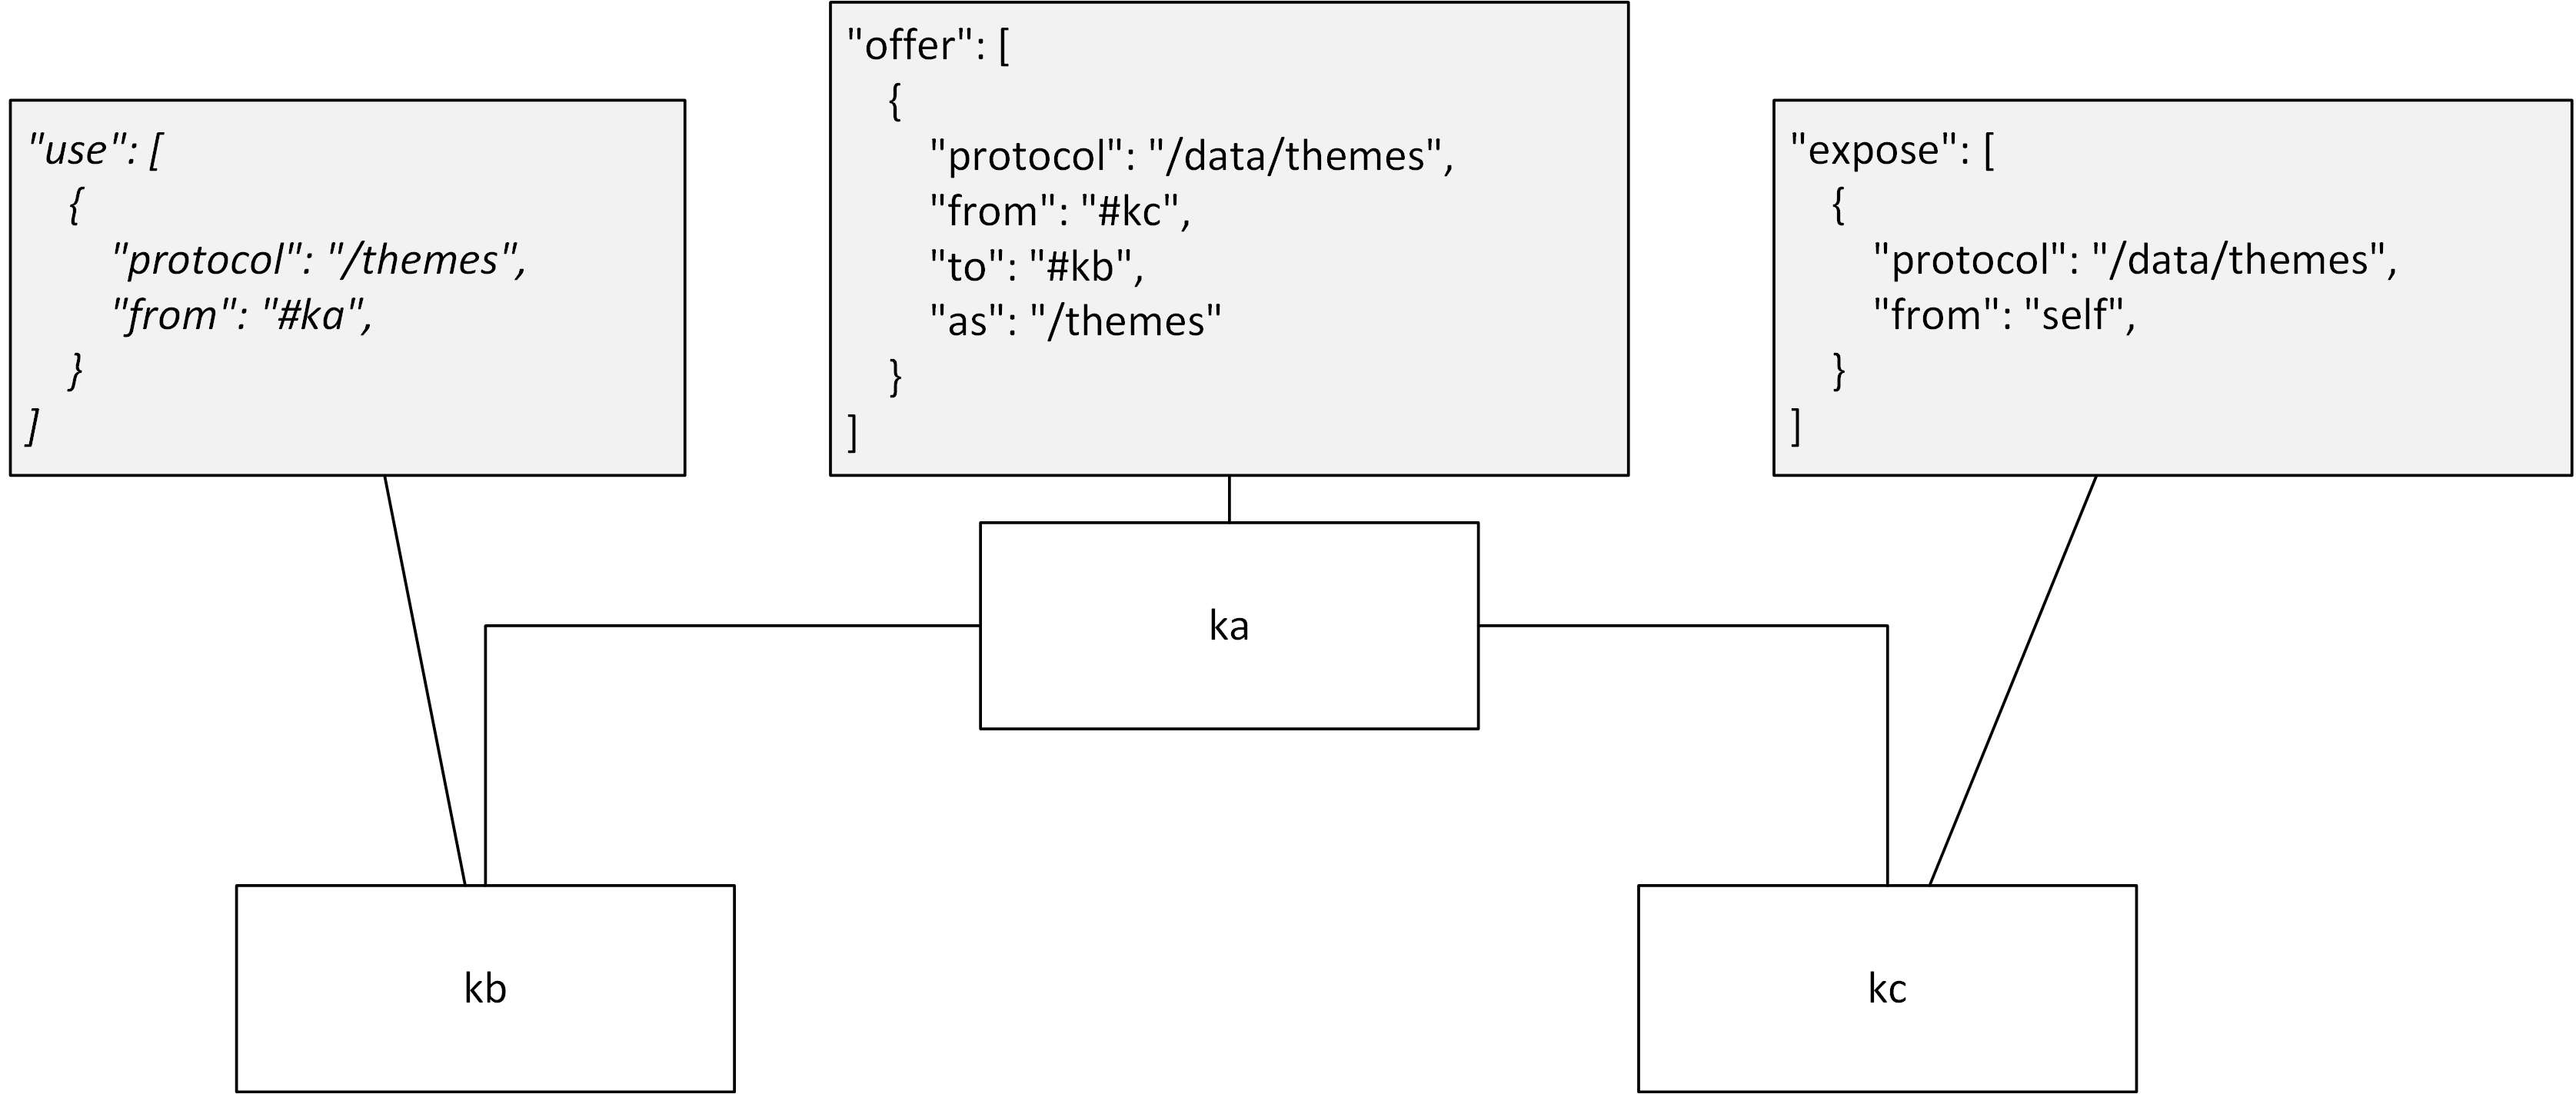
\includegraphics[width=1\textwidth]{figure/Capability_Routing}
	\caption[Kurzform vom Bild]{Graphische Darstellung des Capability Routing der Komponenten ka, kb und kc mit einem Ausschnitt aus den jeweiligen Komponentenmanifesten.}
	\label{abb:capabilityRouting}
\end{figure}
Capabilities können zugänglich gemacht, weitergeleitet und benutzt werden. Welche Komponente was mit welcher Capability macht, wird im Komponenten Manifest der Komponente angegeben. Wenn eine Komponente die Capabilities einer anderen Komponente nutzen möchte, kann sie dies mittels des use Schlüsselwortes im Komponenten Manifests angeben. Hier muss die Komponente den Typ der Capability sowie den Pfad zur Capability angeben, unter dem die Capability freigegeben wurde. Optional kann der Pfad im Komponenten Manifest mittels dem Schlüsselwort as auf einen anderen Pfad geleitet werden. Komponenten können mittels dem Schlüsselwort expose eine Capability an ihre Eltern weiterleiten und mittels offer an ihre Kinder Komponenten. Das Routing der Capabilites wird in Abbildung \ref{abb:capabilityRouting} genauer veranschaulicht. In diesem Beispiel gibt die Komponente kc ein FIDL-Protokoll unter dem Pfad /data/themes frei, während die Komponente ka dieses Protokoll an kb weiterleitet, indem sie es mittels offer ihrer Kind Komponente zur Verfügung stellt, dabei ändert sie den Pfad mittels as auf /themes. 

\subsection{Vergleich zu Komponenten}
Da der Zircon Kernel nur ein Minimum an Diensten zur Verfügung stellt, ist es möglich das Fuchsia System durch das Hinzufügen, Updaten oder Löschen von Komponenten so zu konfigurieren, dass es auf den jeweiligen Anwendungszweck angepasst ist. Ein hinzufügen einer neuen Komponente bedeutet also auch immer, dass der Funktionsumfang des Gesamtsystems erweitert wird.

Durch die Verwendung von Komponenten hat Fuchsia den Vorteil, dass einzelne Funktionen des Systems voneinander getrennt sind. Dies ermöglicht es, dass einzelne Funktionen einfach geupdatet werden können, solange das Interface für die FIDL Schnittstelle gleich bleibt. Es kann also, anders als bei Android bisher, das Problem umgangen werden, dass Google ein Update für das Android System veröffentlicht, dieses jedoch nicht alle User erreicht, da die Hersteller der Geräte die Updates nicht mehr auf ihre Geräte anpassen. Für ChromeOs hat Google bereits eine einfachere Methode entwickelt, um Updates zu installieren. ChromeOs lädt beim Booten das System von einer Partition, während des Betriebes werden mögliche Updates heruntergeladen und auf eine zweite Partition persistiert. Wenn das System neu gestartet wird, wechselt ChromeOs automatisch auf die Partition, die einen neueren Systemstand enthält. Gelingt dies, so wird der alte Stand mit dem neuen überschrieben, anderenfalls findet ein Fallback auf den alten Stand statt und das Update wird erneut heruntergeladen. Google kann im Falle von Fuchsia die Logik innerhalb von Komponenten beliebig austauschen, ohne dass dazu das gesamte System geupdatet werden muss oder Anpassungen durch den Hersteller des Gerätes notwendig wären. Somit ist es nicht mehr notwendig das System neu zu starten, wie es bei ChromeOs der Fall ist und es können trotzdem Fallbacks auf ältere Versionen einer Komponente durchgeführt werden, da das Interface der Komponente immer gleich bleibt. \cite{ChromeOs.Update}

Durch die Kapselung in Komponenten, werden die Auswirkungen, die durch fehlerhafte Komponenten entstehen können, möglichst gering gehalten, da eine Komponente nur so viele Zugriffe auf andere Komponenten hat, wie sie unbedingt benötigt, um Fehlerfrei funktionieren zu können. Dieses Prinzip wird auch Principle of Least Privilege genannt und sorgt im allgemeinen für eine bessere Stabilität des Systems, sowie eine geringere Angriffsoberfläche, sollte es durch den Fehler zu einem Sicherheitsvorfall kommen können.\cite{Android.Security.PoLP} Bei einem Fehler in einer Komponente muss das System die entsprechende Komponente einfach neu starten und die Funktionalität, die die Komponente zur Verfügung gestellt hat, kann weiter genutzt werden.

Da Fuchsia mittels der oben erläuterten Runner Komponenten in beliebigen Programmiersprachen ausführen kann, ist es einfacher für Entwickler in die Entwicklung von Komponenten für Fuchsia einzusteigen, da sie wahrscheinlicher eine Programmiersprache beherrschen, die von Fuchsia unterstützt wird. Während für Android nur Apps unterstützt werden, die in Kotlin oder Java entwickelt wurden. Außerdem muss beim Entwickeln einer neuen Komponente kaum auf die bereits vorhandene Logik im System geachtet werden, da durch das fest definierte Interface bereits Teile der Implementierungsdetails definiert sind. Das Testen einer einzelnen Komponente ist zudem einfacher umsetzbar, als Tests zu erstellen, die auf alle möglichen Zustände des Gesamtsystems angepasst sein müssen.

Da Android auf den Linux Kernel setzt, läuft der gesamte Kernel in einem einzigen Adressbereich und ein Fehler in diesem Kernel kann zur Folge haben, dass das gesamte System in einen Fehlerzustand wechselt. Jedoch wird durch den einzelnen Adressbereich auch die Menge der IPC Kommunikation verringert, da nicht für jeden Datenaustausch eine Verbindung zwischen zwei Prozessen hergestellt werden muss, sondern innerhalb desselben Prozesses kommuniziert werden kann, dies wirkt sich im allgemeinen positiv auf die Performance von monolithischen Kernels aus.

Die Testbarkeit des unter Android verwendeten Linux Kernels wird durch die Komplexität des Systems erheblich erschwert, während Fuchsia, wie oben erwähnt, nur einzelne Funktionalitäten einer Komponente testen muss, müssen im Linux Kernel immer alle möglichen Zustände des Systems getestet werden, die Auswirkungen auf die zu testende Funktion haben könnten.

Der Linux Kernel bündelt alles innerhalb eines großen Kernels, der, so denn die Funktionalität für einen Anwendungsfall eingeschränkt werden soll, neu kompiliert werden muss. Dies ist bei Fuchsia nicht notwendig, durch den Komponentenansatz sind nur die notwendigsten Dienste vorhanden und alles was zusätzlich benötigt wird, kann dynamisch dazu geladen werden.

Unter Android gibt es eine ähnliche Interface Sprache, wie FIDL, um die Kommunikation zwischen Clients und Services zu definieren. Unter Android heißt diese Sprache Android Interface Definition Language kurz AIDL, sie definiert, ähnlich wie bei FIDL, ein Interface zur Inter Prozess Kommunikation. Im Gegensatz zu FIDL setzt AIDL jedoch auf die Syntax, die auch in Java Interfaces verwendet wird, während Fuchsia eine C++ ähnliche Syntax verwendet und dabei mehr Strukturen unterstützt als AIDL. Dies bedeutet aber auch, dass AIDL im Gegensatz zu FIDL nur einen Rückgabewerte unterstützt und nicht wie FIDL beliebig viele.
\section{Treiber}
\subsection{Verwaltung und Zugriff}
Treiber in Fuchsia werden hierarchisch organisiert und möglichst kleinteilig pro Gerät gesplittet, somit wird eine unnötige Duplizierung von Programmcode verhindert.

Das Treiber-Framework in Fuchsia enthält unter anderem einen Gerätekoordinator, dieser verwaltet eine Baumstruktur, die den Aufbau der Abhängigkeiten zwischen den einzelnen Treibern darstellt. So kann beispielsweise ein USB-Treiber als Elternknoten an einem PCI-Gerät hängen und selbst wieder einen Soundkarten Treiber als Kind haben, da an diesem PCI-Slot eine USB-Soundkarte hängt. Der Gerätemanager durchsucht /boot/driver und /system/driver nach Treibern, jeder dieser Treiber ist als Dynamic Shared Object (DSO) implementiert. Damit der Geräte Koordinator bestimmen kann, welcher Treiber für welches Gerät verwendet werden kann, muss jeder Treiber eine Binding-Routine implementieren, die bestimmt, für welche Geräte dieser Treiber eingesetzt werden kann. Meist wird dazu die Vendor ID (VID) und Device ID (DID) verwendet, da diese in Kombination einzigartig für ein Gerät sind. \cite{Fuchsia.Drivers}

Der Treiberbaum hat initial einen Root-PCI-Driver als Wurzel, dieser geht davon aus, dass sich in dem System ein PCI fähiges Gerät befindet, wenn es gefunden wird, dann wird es an diesen Treiber gebunden. Für alle Geräte, die wiederum physisch mit dem PCI Gerät verbunden sind, schaut der Gerätekoordinator in definierten Verzeichnissen nach, ob dort ein Treiber gefunden werden kann, dessen Binding Funktion für diese VID und DID ein positives Ergebnis liefert. Jeder Pfad von der Wurzel des Baumes bis zu jedem Blatt wird vom Gerätekoordinator als Gerät betrachtet. \cite{Fuchsia.Drivers.Composite}

Basierend auf einer Systemrichtlinie splittet der Gerätekoordinator den Baum in einzelne Teilbäume, die jeweils innerhalb eines Geräte-Host-Prozesses (devhost) ausgeführt werden, durch die Teilung der Gerätetreiber in einzelne Gruppen soll eine höhere Stabilität und Sicherheit erzielt werden können, da die Treiber getrennt voneinander ausgeführt werden.\cite{Fuchsia.Drivers.Composite}

Treiber können Metakommunikation für das Gerät bzw. den Treiber mittels eines FIDL-Protokolls definieren. Das Lesen bzw. Schreiben von Daten an ein Gerät ist wie ein Lesezugriff bzw. Schreibzugriff auf eine Datei realisiert. Das Gerät ist dabei unter /dev/ gemounted.
\subsection{Vergleich Treiber}
Der Linux Kernel trennt Treiber nicht in einzelne Prozesse, sondern lässt, bedingt durch den monolithischen Kernel alle Treiber innerhalb desselben Prozesses laufen. Dies hat zur Folge, dass ein Fehler in einem Treiber zu einem System Absturz führen oder eine Sicherheitslücke zu root Zugriff führen kann. Linux unterteilt Treiber in drei Kategorien: byteorientierte Geräte (z.B. Tastaturen), blockorientierte Geräte (z.B. Festplatten) und paketorientierte Geräte. Byteorientierte Geräte können nur jeweils ein Zeichen auf einmal ausgeben oder einlesen und sind als Dateien in das Dateisystem unter /dev/ in Linux eingebunden. Blockorientierte Geräte können nur ein vielfaches der spezifizierten Blockmenge lesen bzw. schreiben. Sie sind über einen Pfad im Dateisystem von Linux erreichbar, der als lesbare Datei dargestellt wird. 

Byteorientierte und blockorientierte Treiber werden unter Linux im chrdev bzw. blkdev Vektor gespeichert, sobald ein Gerät erkannt wird, wird der entsprechende Treiber in den Vektor eingefügt und ab dann werden die Major und Minor Nummer zur Identifizierung des Gerätes verwendet, wobei die Major Nummer den Type des Gerätes angibt (z.B. tty) und die Minor Nummer die einzelne Instanz des Gerätes identifiziert. Der Zugriff auf die Geräte erfolgt dann über eine Datei im Pfad /dev und mittels den regulären Systemcalls für Dateien können Daten von dem Gerät gelesen und an das Gerät gesendet werden.

Das Treibermanagement in Fuchsia und Linux unterscheidet sich also in zwei Aspekten. Fuchsia unterhält einen Baum, indem alle Geräte als Blätter repräsentiert werden, wohingegen Linux die Geräte in drei Klassen unterteilt und für jede Klasse einen eigenen Vektor mit den jeweiligen Geräten in dieser Klasse pflegt.

Außerdem sind Treiber unter Fuchsia im Userspace in einzelne Prozesse gekapselt, während Linux alle Treiber im Kernelspace ausführt. Der Userspace Ansatz hat zum Vorteil, dass die Auswirkungen von Bugs im Treiber oder aber auch absichtlich Manipulierte Treiber nur innerhalb ihres Prozesses Schaden anrichten können und keine Auswirkungen auf den Kernel an sich haben, wie es etwa bei Linux der Fall ist. Beim Linux Ansatz hingegen ist die Performance potenziell  besser, da kein Kontextwechsel zwischen Kernelspace und Userspace notwendig ist, deshalb startet Fuchsia nicht für jedes Gerät einen neuen Prozess, sondern kapselt mehrere Geräte in einen Prozess.

\section{Dateisystem}
\label{sec:Dateisystem}
\subsection{Dateisystem Architektur und Dateisystem}
Zircon hat kein eigenes Dateisystem, sondern setzt darauf, dass ein Dateisystem im Userspace als Prozess zur Verfügung gestellt wird. Dadurch wird es theoretisch möglich, dass das Dateisystem während des laufenden Betriebes ausgetauscht und geupdatet werden kann. Diese Architektur setzt jedoch voraus, dass die Interaktion mit dem Dateisystem auf ein Interface beschränkt ist, dieses wird in Fuchsia mittels FIDL definiert. \cite{Fuchsia.FIDL.io}\cite{Fuchsia.FIDL.io2} Das Kommunikationsmodell für die Interaktion mit dem Dateisystem findet, da es sich immer um eine Kommunikation zwischen zwei Benutzerprozessen handelt, über Channels statt, wodurch ein Server/Client System entsteht. Der Prozess, der das Dateisystem zur Verfügung stellt, entspricht dabei einem Server und die Prozesse, die über die Channels, auf diesen Serverprozess zugreifen, um das Dateisystem zu nutzen, entsprechen in diesem Modell den Clients. Eine Konsequenz aus diesem Konzept ist, dass eine Datei nicht mittels Systemcall geöffnet werden kann, sondern erst eine IPC Verbindung durch einen Fuchsia Channel \cite{Fuchsia.Kernel.KernelObjects} zwischen den Prozessen hergestellt werden muss, dadurch kommt es zu zwei Kontextwechseln (Userspace von Prozess A in Kernelspace in Userspace von Prozess B). Dateisysteme haben typischerweise 2 Handels, eines, um mit dem Dateisystem selbst zu kommunizieren, und ein optionales, um mit dem Gerät zu kommunizieren, auf dem das Dateisystem gespeichert wird. \cite{Fuchsia.Storage}

\textbf{FVM (Fuchsia Volume Manager)} ist eine Mittelschicht zwischen existierenden blockbasierten Geräten und einem Dateisystem. Es bietet die Möglichkeit Partitionen zu erstellen, die in ihrer Größe ein Vielfaches der Blockgröße des Gerätes besitzen, und sich dabei über mehrere Speichergeräte hinweg erstrecken können. Dies ermöglicht es, dass Dateisysteme nicht fest an die Größe des Speichergerätes gebunden sind, sondern flexibel ihre Größe ändern können. Um dies zu realisieren bietet der Fuchsia Volume Manager ein Mapping zwischen den physisch existierenden Speicherblöcken und einer Virtuellen Partition, somit kann eine Partition vergrößert werden, indem mehr physische Speicherblöcke dieser Partition zugewiesen werden, andersherum kann eine Partition verkleinert werden, indem Speicherblöcke aus dem Mapping entfernt werden. Jeder Speicherblock kann entweder einer Partition zugewiesen sein oder frei sein.\cite{Fuchsia.Storage}

Fuchsia nutzt aktuell vier verschiedene Arten von Dateisystemen.\cite{Fuchsia.Storage}

\textbf{MemFS} (Memory Filesystem) wird meist für Temporäre Daten genutzt und ist ein Dateisystem, dass komplett im Memory existiert, somit also nicht persistiert wird. Dieses Dateisystem wird zum Beispiel für das bootfs Protokoll genutzt.

\textbf{MinFS} ist ein persistentes Dateisystem, dass dem von Unix sehr stark ähnelt, dabei sind maximal Dateien bis zu einer Größe von 4 Gigabyte möglich. Dieses Dateisystem benötigt das weiter oben beschriebene Handle, das einen direkten Zugang auf das Gerät ermöglicht, auf dem die Daten persistiert werden.

\textbf{Blobstore} ist ein Dateisystem, dass auf „Write once then read-only“ optimiert wurde. Es besitzt eine flache Hierarchie, das bedeutet, dass alle Daten im Root Verzeichnis liegen. Der Blobstore wird zur Speicherung und Integritätsüberprüfung von Anwendungspaketen verwendet. Damit die Integrität dieser Pakete gesichert ist, wird über alle Dateien ein Merkle-Tree gespannt, also eine auf kryptographischen Hashfunktionen basierende Integritätssicherung, um Manipulationen an den Anwendungspaketen auszuschließen.

\textbf{ThinFS} ist eine in GO implementierte Version des FAT-Dateisystems, die von Fuchsia verwendet wird, um auf FAT-Dateisysteme zugreifen zu können. Da FAT immer noch häufig für USB-Sticks und EFI-Partitionen verwendet wird.
\subsection{Cloudunterstützung}
\label{sec:Ledger}
Ledger ist ein auf Schlüsselwertpaaren basierender verteilter Speicher. Der Ledger erlaubt es basierend auf diesen Schlüsselwertpaaren Daten über einen Cloudspeicher mit anderen Geräten zu synchronisieren. Ein Eintrag besteht aus einem 16 Byte Schlüssel und einem beliebig großen Byte Wert, der zum Zeitpunkt dieser Arbeit nur durch die Nachrichtengröße für FIDL Nachrichten limitiert ist.

Der Ledger selbst besteht aus drei Ebenen. Auf der ersten Ebene befindet sich der Lokale Client, dieser stellt eine FIDL API für Komponenten zur Verfügung über die Änderungen, Löschungen und Abfragen von einzelnen oder mehreren Einträgen möglich sind. Wenn es durch die Änderungen, die eine Komponente über die API angefragt hat zu einem Konflikt kommt, versucht der Client diesen Konflikt zu lösen, indem er die Strategie verwendet, die vorher von der Komponente angegeben wurde, wenn diese nicht möglich ist, wird die Anfrage zurück an die Komponente geleitet. Wenn die Anfrage nicht zu einem Konflikt führt, werden die Änderungen auf die zweite Ebene weitergeben. Auf der zweiten Ebene werden die Daten im Storage mittels eines atomaren Commits persistiert. Der Commit-Verlauf jeder Seite kann, ähnlich wie bei GIT, als DAG dargestellt werden. Der Storage speichert für jeden Commit zusätzlich die Metadaten für die Einträge und sortiert sie in einen B-Baum ein. Wenn der Commit persistiert wurde, benachrichtigt der Storage die dritte und letzte Ebene, den Cloud Sync, dieser lädt den neuen Commit in die Cloud und stellt die Daten damit für die anderen Geräte zur Verfügung. Außerdem achtet der Cloud Sync auf Änderungen im Cloud Speicher und lädt die neuen Einträge herunter und pflegt sie in den Speicher ein, damit die Lokale Kopie und der Cloud Speicher möglichst immer dieselben Daten enthalten. \cite{Fuchsia.Ledger}

Der Ledger unterstützt zwei verschiedene Betriebsmodi zum einen den Guest Mode und zum anderen den Regularmode. Im Guestmode hat der Ledger keine aktive Verbindung zur Cloud und speichert die Daten lediglich lokal. Im Regularmode hat der Ledger eine aktive Verbindung zur Cloud und synchronisiert alle Geräte, die mit demselben Benutzerkonto verbunden sind.
\subsection{Vergleich Filesystems}
\label{sec:vglFileSystems}
Unter Android und ChromeOs ist das Dateisystem, wie bei Linux üblich, in den Kernel des Betriebssystems integriert. Dies hat zur Folge, dass zusätzliche Dateisysteme nicht, wie etwa bei Fuchsia durch neue Komponenten im Userspace hinzugefügt werden können, sondern dass ein Treiber für das entsprechende Dateisystem im Kernel installiert werden muss. Dies lässt sich auf den meisten Android Geräten nicht realisieren, ohne dass die Sicherheitsmechanismen des Geräteherstellers umgangen werden, da die Android Version auf den Geräten der Hersteller meist nur im Nutzermodus ausgeführt werden kann. Android unterstützt in der Regel ext4 und ext3 für den internen Speicher des Gerätes und hat eine Unterstützung für exFAT und FAT32, um auch auf externen Speicher, wie z.B. SD-Karten zugreifen zu können, ähnlich, wie Fuchsia mit ThinFS eine eigene Implementierung von FAT besitzt, um Zugriff auf USB-Sticks und SD-Karten zu ermöglichen.

In früheren Versionen von Android konnten alle Apps auf alle Daten von allen anderen Apps und zum Teil auch auf Systemdateien zugreifen. Mit Android 10 bzw. API Level 29 hat Google jedoch eine zu Fuchsia ähnliche Struktur des Speichers integriert. Die MediaStore API erlaubt den Zugriff auf Mediadateien von anderen Apps nur noch, wenn die App vom Benutzer explizit das Recht bekommen hat auf den Speicher des Systems zuzugreifen. Über das Storage Access Framework kann nur auf Dateien zugegriffen werden, die der Nutzer über einen File Picker explizit für die App zur Verfügung stellt, alle anderen Dateien, die auf dem Gerät gespeichert sind, bleiben für die App verborgen. Fuchsia trennt, wie in Kapitel \ref{sec:Components} beschrieben, den Speicher der einzelnen Komponenten voneinander, während das Speicherkonzept von Android erst in den neueren Versionen diese Trennung erhalten hat. Ebenso wird der Speicher von einzelnen Android Apps erst in den neueren Android Versionen getrennt. \cite{Android.Storage.Overview}

Der in Kapitel \ref{sec:Ledger} beschriebene Cloudspeicher Ledger ist in dieser Form nicht in Android verfügbar, Android besitzt jedoch einen lokalen Schlüssel-Wert-Speicher, der ähnlich, wie bei Fuchsia dazu genutzt werden kann, um die Einstellungen einer App zu speichern, jedoch hat dieser Speicher unter Android keine Synchronisationsfunktion, wie es mit Ledger möglich ist. \cite{Android.Storage.Overview} Der neue File Picker kann unter Android verwendet werden auf Cloudspeicher zuzugreifen, ohne dass die App merkt, dass es sich dabei um eine Datei in der Cloud handelt und nicht auf dem Gerät selbst, somit wird eine Transparenz des Speicherorts erzeugt. \cite{Android.Storage.DocumentProvider}

ChromeOS setzt ähnlich, wie Fuchsia, auf einen Cloudspeicher, um die Daten der Nutzer zu speichern und über Geräte hinweg zu synchronisieren. Ebenso ist es mit ChromeOs möglich, dass der Benutzer das System komplett auf den Werkszustand zurücksetzen kann und anschließend, indem er sich in sein Google Konto einloggt, alle Apps und Einstellungen wiederherstellen kann. Da ChromeOs darauf ausgelegt ist, dass möglichst alle Daten in einer Cloud gespeichert werden, existieren die meisten Daten nur lokal auf dem Gerät, um eine schnelle Verfügbarkeit der Daten zu gewährleisten.
\section{Zusammenfassung}
Fuchsia bietet mit dem neu geschriebenen Zircon Kernel durch das Microkernel Konzept einen wesentlich schlankeren Kernel als Android und ChromeOs mit ihrem Linux Kernel. Dies macht Fuchsia in Verbindung mit dem Komponenten Ansatz zu einem System, dass sehr flexibel an ein Anwendungsgebiet angepasst werden kann. So kann das System auf fast allen Geräteklassen verwendet werden; von einem IoT Gerät bis hin zu einem vollwertigen Desktop System ist alles denkbar. Je nach Geräteklasse kann das System mit den Komponenten ausgestattet werden, die für das jeweilige Gerät benötigt werden. Somit wird es einfacher Software für die entsprechenden Geräte zu schreiben, da alle Geräte auf demselben Betriebssystem basieren, kann eine Komponente, die beispielsweise den Netzwerkzugriff ermöglicht, einfach auf allen Geräteklassen verwendet werden, wobei sich nur der Treiber für das Netzwerkgerät im entsprechenden Gerät unterscheidet.

Updates für das Android System sind aktuell davon abhängig, dass die Gerätehersteller das Update für ihre Geräte anpassen und anschließend an ihre Nutzer verteilen, da Gerätehersteller meist darauf verzichten Updates für Ihre Geräte über einen längeren Zeitraum anzupassen, führt dies dazu, dass viele Geräte keine Updates erhalten und somit unnötig zu Elektroschrott verkommen. Mit Fuchsia kann diese Problematik weitestgehend entschärft werden, da sich nur die notwendigste Funktionalität in Zircon befindet, können die Komponenten, die die weiteren Funktionen zur Verfügung stellen einfach ein Update erhalten, sogar ohne, dass dazu ein Neustart des Systems notwendig wäre.

Android Apps können in Java oder Kotlin entwickelt werden. ChromeOs Apps bzw. Erweiterungen werden meist in C++ oder in Websprachen entwickelt. Fuchsia Komponenten sind im Gegensatz dazu theoretisch nicht an eine feste Programmiersprache gebunden, da wie in Kapitel \ref{sec:FIDL} beschrieben, Komponenten in jeder Programmiersprache entwickelt werden können, für die ein entsprechender Runner existiert. Aktuell beschränkt sich die Auswahl auf C++, C, Dart, Rust und Go, da jedoch nur ein Runner für eine Sprache entwickelt werden muss, um die Sprache zu unterstützen, kann damit gerechnet werden, dass zum Zeitpunkt des offiziellen Releases von Fuchsia weitaus mehr Sprachen unterstützt werden. Somit müssen Entwickler keine neue Programmiersprache erlernen, um für Fuchsia Komponenten entwickeln zu können, sondern können die Programmiersprachen verwenden, die sie bereits kennen.

Wie in Kapitel \ref{sec:vglFileSystems} beschrieben, nähert sich das Dateisystem unter Android an das Konzept in Fuchsia an. Durch den Ansatz, den Fuchsia verfolgt, indem jede Komponente seinen eigenen Speicher hat und nur durch explizite Freigabe Daten auch von anderen Komponenten, erreichbar sind, bietet Fuchsia per Design größere Sicherheit als Android. Komponenten können mit diesem Design nicht auf die Daten von anderen Komponenten zugreifen, die beispielsweise private Daten des Nutzers enthalten. Durch Ledger hat Fuchsia einen integrierten Cloudagent, der Daten zwischen Geräten austauschen kann, dieser kann es dem Benutzer des Systems erleichtern bei Neuanschaffung eines Gerätes die Einstellungen und Daten des alten Gerätes auf das neue Gerät zu erleichtern oder aber die Arbeit mit mehreren Geräten zu erleichtern.
\bibliography{referenzen}
\bibliographystyle{unsrt}

\end{document}
